% !TeX root = Main.tex

Pro demonstraci simulačního modulu aplikace Agros2D, jehož řešené rovnice jsou popsány v kapitole \ref{kap:Simulace}, je zde uveden příklad z oboru vysokofrekvenční techniky. 

\section{Zadání úlohy}
Geometrické rozměry pravoúhlého vlnovodu R100 jsou následující. Vstup má $a = 22,86 \unit{mm}$, $b = 10,16 \unit{mm}$ a celková délka vlnovodu $l$ je $0,17 \unit{m}$. Vlnovodem se šíří dominantní elektické vidy a vnitřním materiálem je vzduch. 
\begin{enumerate}
\item[a)] Určete mezní kmitočet vlnovodu R100 a rozhodněte, zda se může šířit vlna o frekvenci $f_0 = 9 \unit{GHz}$. Následně proveďte rozbor pomocí programu Agros2D pro tento kmitočet. 
\item[b)] Uvažujte změnu geometrie tak, že ve vzdálenosti $0,076 \unit{m}$ od vstupu je vlnovod skokově zúžen, rozměr širší strany $a$ se zmenší na $9 \unit {mm}$. Délka zúžení je $5 \unit{mm}$. 

Určete mezní kmitočet zúžené části a proveďte programovou analýzu upraveného vlnovodu pro následující frekvence:  $f_1 = 9 \unit{GHz}$, $f_2 = 12,4 \unit{GHz}$ a $f_3 = 17,5 \unit{GHz}$.
\end{enumerate}

\section{Řešení varianty a) vlnovod R100}
Mezní kmitočet vlnovodu R100 se vypočte pomocí vztahu (\ref{rce:evlny_vlnovody_mezni_frekvence})
\begin{displaymath}
f_{m1} = \frac{c}{2\pi\sqrt{\varepsilon_{r}\mu_{r}}}\cdot\sqrt{\bigg(\frac{\pi}{a}\bigg)^{2}} = \frac{3\cdot 10^{8}}{2\pi\sqrt{1}}\cdot\sqrt{\bigg(\frac{\pi}{22.86\cdot 10^{-3}}\bigg)^{2}} = 6.56 \unit{GHz}.
\end{displaymath}
Zadaná frekvence $f_0$ je vyšší než mezní kmitočet a proto se vlna může vlnovodem šířit.

\subsection*{Geometrie a okrajové podmínky}
Dle zadaných rozměrů zakreslíme geometrii vlnovodu dle postupu, který je uveden v příloze \ref{kap:tutorial}. 
\begin{figure}[!h]
	\centering
	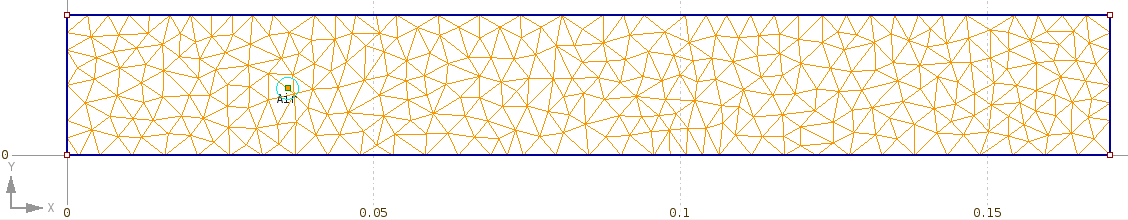
\includegraphics[width=15cm]{priklad_R100_diskretizace.png}
	\caption{Diskretizace řešené oblasti vlnovodu trojúhelníkovými prvky}
	\label{obr:priklad_R100_diskretizace}
\end{figure}
Oblast na obrázku \ref{obr:priklad_R100_diskretizace} pokryjeme diskretizační sítí, u které definujeme, pomocí značky oblasti použitého materiálu, maximální obsah prvku na $0,00001 \unit{m^{2}}$. Dále je pro řešení potřeba specifikovat okrajové podmínky na příslušných hranicích.
\begin{itemize}
\item $E = 0$ - Představuje podmínku označovanou jako \uv{prefect electric conductor} vyjádřenou pomocí intenzity elektrického pole. Zadáme ji na obě podélné hranice na obrázku \ref{obr:priklad_R100_diskretizace}.
\item $J_{t} = -\frac{1}{\omega\mu}\frac{\partial E}{\partial n_{0}} = 10 + \mj10$ - Zadání povrchového proudu vstupujícího do vlnovodu. Přísluší k levé hranici, dle obrázku\ref{obr:priklad_R100_diskretizace}.
\item $-\frac{1}{\omega\mu}\frac{\partial E}{\partial n_{0}} = \sqrt{\frac{\varepsilon - \mj\sigma/\omega}{\mu}}E$ - Nakonec na pravou stranu vlnovodu přiřadíme impedančně přizpůsobenou hranici.
\end{itemize}
Po spuštění řešení pro zadanou frekvenci $f_0 = 9\unit{GHz}$ získáme pomocí postprocesoru následující výsledky. První dva obrázky, tj. \ref{obr:priklad_R100_Ere} a \ref{obr:priklad_R100_E}, popisují intenzitu elektrického pole. Dále obrázky \ref{obr:priklad_R100_Hre} a \ref{obr:priklad_R100_H} znázorňují intenzitu magnetického pole. Nakonec obrázek \ref{obr:priklad_R100_N} je výsledkem rozložení výkonu dle Poyntingova vektoru na řešené oblasti.
\begin{figure}[!h]
	\centering
	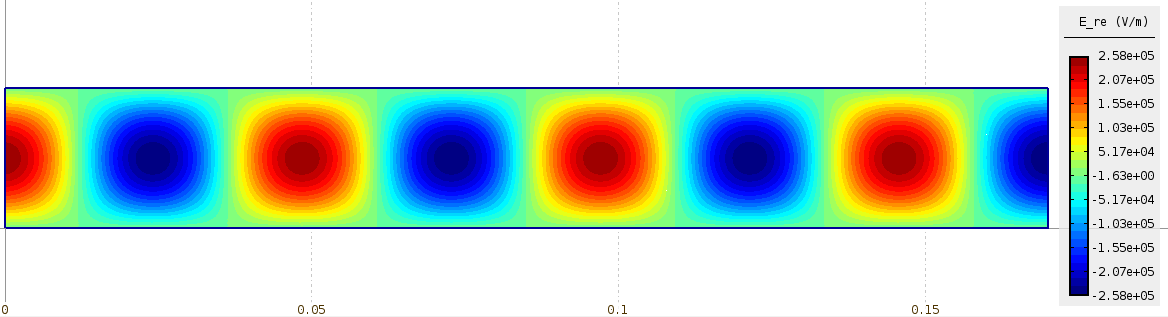
\includegraphics[width=15cm]{priklad_R100_Ere.png}
	\caption{Rozložení reálné složky intenzity elektrické pole.}
	\label{obr:priklad_R100_Ere}
\end{figure}
\begin{figure}[!h]
	\centering
	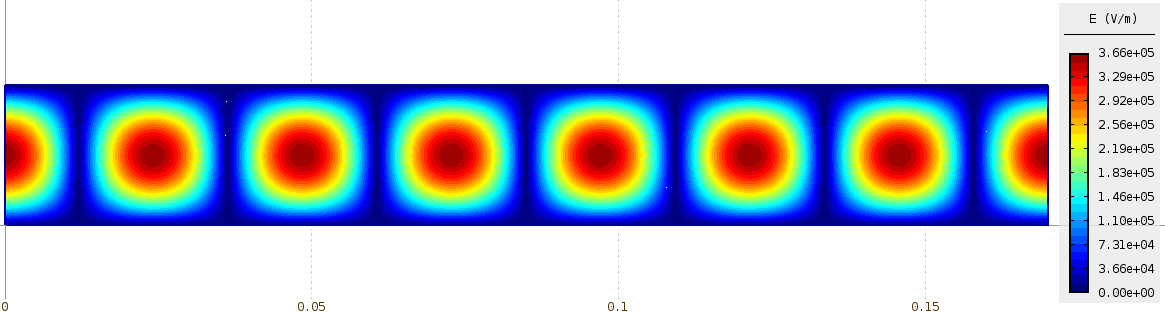
\includegraphics[width=15cm]{priklad_R100_E.png}
	\caption{Modul intenzity elektrické pole.}
	\label{obr:priklad_R100_E}
\end{figure}
\begin{figure}[!h]
	\centering
	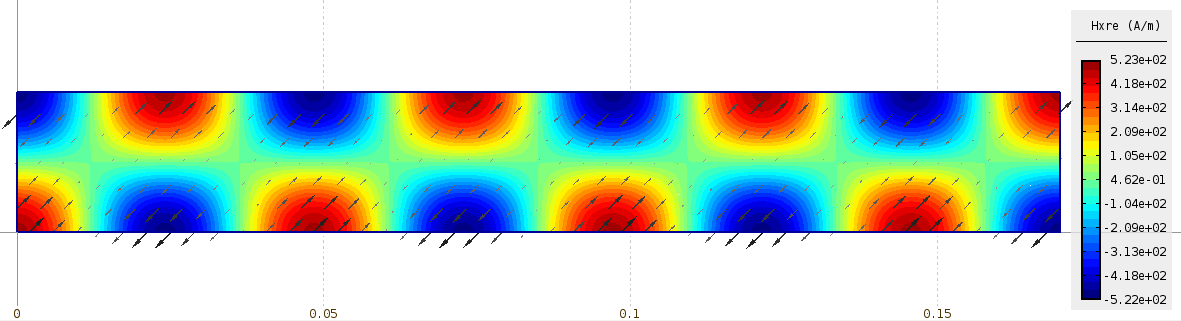
\includegraphics[width=15cm]{priklad_R100_Hre.png}
	\caption{Reálná složka intenzity magnetického pole ve směru $x$ (zobrazené vektory).}
	\label{obr:priklad_R100_Hre}
\end{figure}
\begin{figure}[!h]
	\centering
	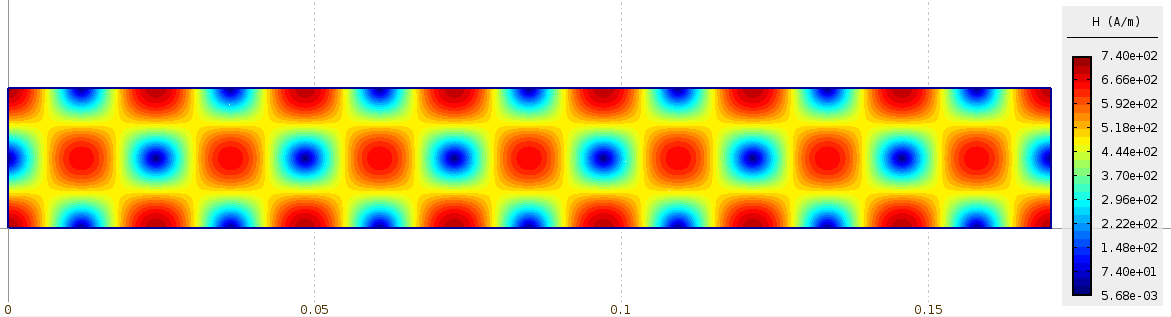
\includegraphics[width=15cm]{priklad_R100_H.png}
	\caption{Modul intenzity magnetického pole.}
	\label{obr:priklad_R100_H}
\end{figure}
\begin{figure}[!h]
	\centering
	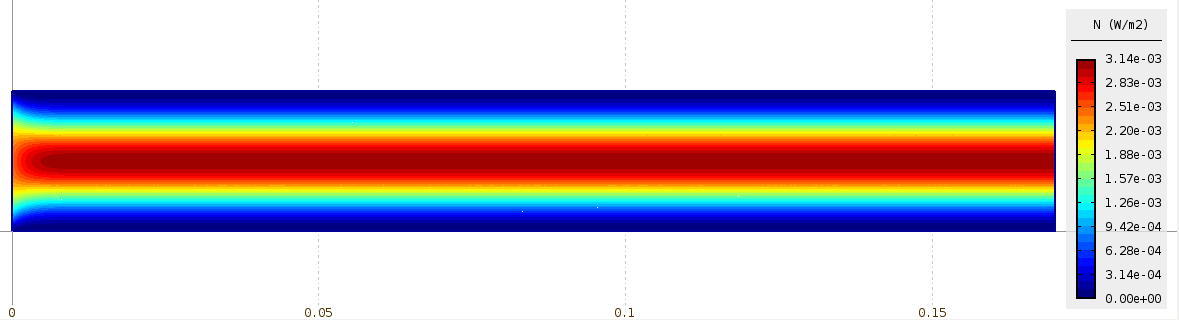
\includegraphics[width=15cm]{priklad_R100_N.png}
	\caption{Rozložení Poyntingova vektoru.}
	\label{obr:priklad_R100_N}
\end{figure}

\section{Řešení varianty b) upravený vlnovod R100}
Opět provedem nejprve výpočet mezního kmitočtu, ale tentokrát pro část vlnovodu zúženou na $9\unit{mm}$
\begin{displaymath}
f_{m2} = \frac{c}{2\pi\sqrt{\varepsilon_{r}\mu_{r}}}\cdot\sqrt{\bigg(\frac{\pi}{a}\bigg)^{2}} = \frac{3\cdot 10^{8}}{2\pi\sqrt{1}}\cdot\sqrt{\bigg(\frac{\pi}{9\cdot 10^{-3}}\bigg)^{2}} = 16.67 \unit{GHz}.
\end{displaymath}
Pro kmitočty v rozmezí $f_{m1}$ až $f_{m2}$ by mělo ve vstupní části vlnovodu dojít ke vzniku vln, které ale budou při průchodu zúženou částí tlumeny. Je to z důvodu existence  podkritického vlnovodu pro kmitočty menší než mezní kmitočet. Tento průběh se dá očekávat pro zadanou frekvenci $f_1$. Naopak pro $f_2$, která je vyšší než vypočtená $f_{m2}$ dojde k průchodu vln do další části.

Po zadání stejných okrajových podmínek a shodného materiálu vlnovodu provedeme analýzu pro změněnou geometrii v aplikaci Agros2D.

\subsubsection*{Frekvence 9 GHz}
Z obrázků \ref{obr:priklad_R100narrow_Ere_9Ghz} a \ref{obr:priklad_R100narrow_Ere_9Ghz_3D} je patrné tlumení elektromagnetické vlny v podkritickém vlnovodu. Vzhledem k nižší frekvenci, než je vypočtená $f_{m2}$, dochází od zúžené oblasti k odrazům a vzniku stojatého vlnění.

Zobrazení dalších veličin plně koresponduje s ověřeným předpokladem. U Poyntingova vektoru (obrázek \ref{obr:priklad_R100narrow_N}) je patrné soustředění výkonu v podkritickém úseku.
\begin{figure}[!h]
	\centering
	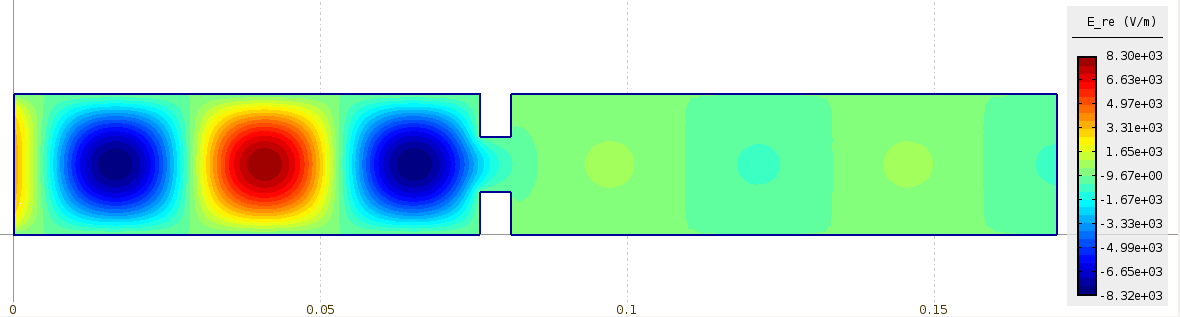
\includegraphics[width=15cm]{priklad_R100narrow_Ere_9Ghz.png}
	\caption{Reálná složka intenzity elektrického pole $E_{z\Re}$ při $f_1 = 9\unit{Ghz}$.}
	\label{obr:priklad_R100narrow_Ere_9Ghz}
\end{figure}
\begin{figure}[!h]
	\centering
	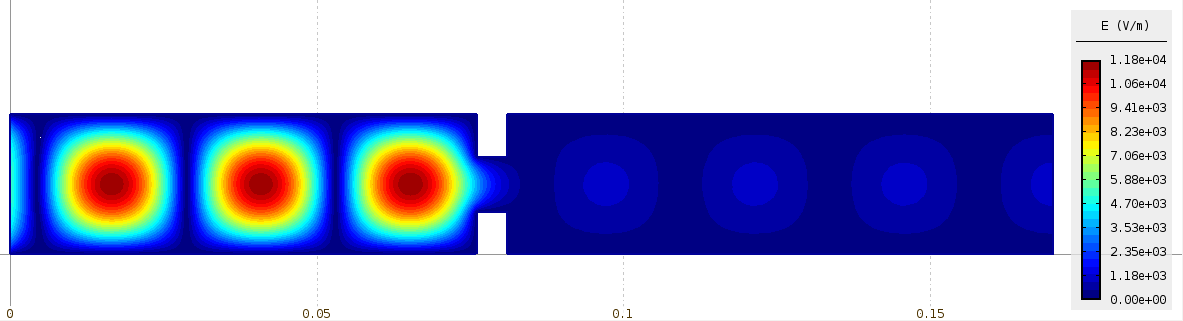
\includegraphics[width=15cm]{priklad_R100narrow_E.png}
	\caption{Modul intenzity elektrického pole $E$ ($f_1 = 9\unit{Ghz}$).}
	\label{obr:priklad_R100narrow_N}
\end{figure}
\begin{figure}[!h]
	\centering
	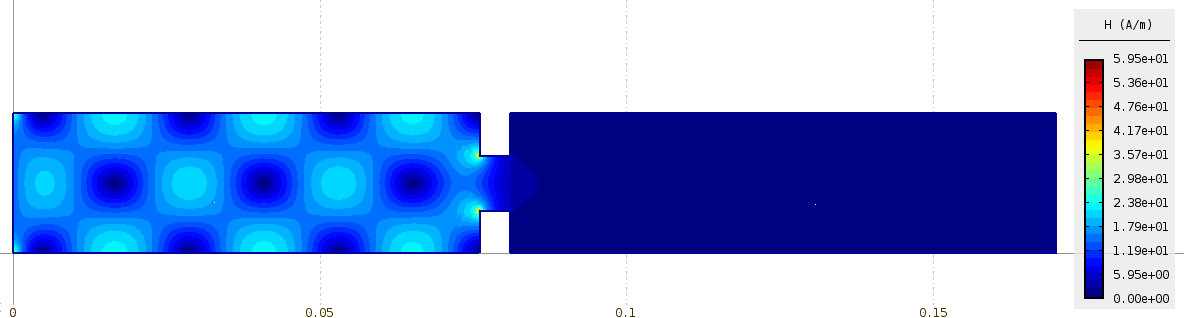
\includegraphics[width=15cm]{priklad_R100narrow_H.png}
	\caption{Modul intenzity magnetického pole $H$ ($f_1 = 9\unit{Ghz}$).}
	\label{obr:priklad_R100narrow_H}
\end{figure}
\begin{figure}[!h]
	\centering
	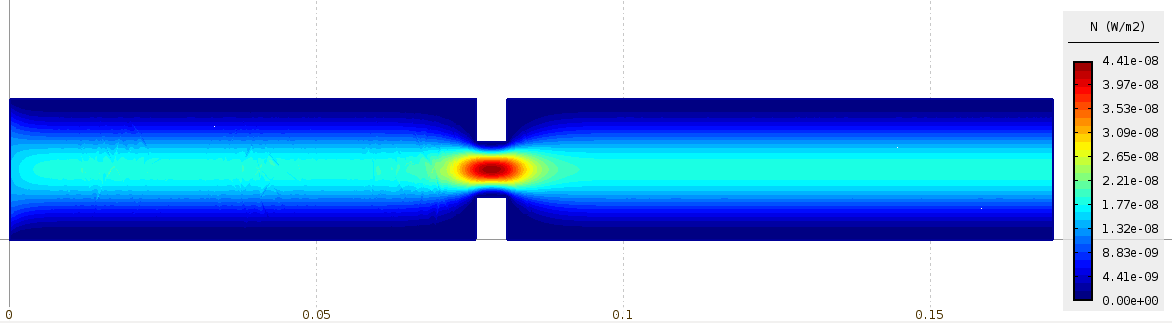
\includegraphics[width=15cm]{priklad_R100narrow_N.png}
	\caption{Poyntingův vektor ($f_1 = 9\unit{Ghz}$).}
	\label{obr:priklad_R100narrow_N}
\end{figure}

\newpage
\subsubsection*{Frekvence 12,4 GHz}
Zvyšováním kmitočtu dochází k pronikání přes podkritický úsek. Ačkoliv je frekvence stále nižší než $f_{m2}$, tak velikost amlitudy vlny v druhé části činí cca $25 \%$ amplitudy vlny vstupující.
\begin{figure}[!h]
	\centering
	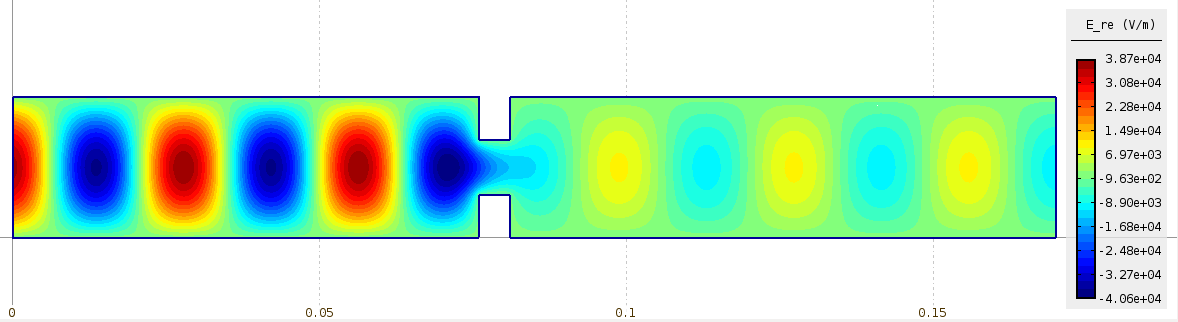
\includegraphics[width=15cm]{priklad_R100narrow_Ere_12Ghz.png}
	\caption{Rozložení $E_{z\Re}$ pro $f_2 = 12,4\unit{Ghz}$.}
	\label{obr:priklad_R100narrow_Ere_12Ghz}
\end{figure}

\subsubsection*{Frekvence 17,5 GHz}
Při tomto kmitočtu, který je vyšší než mezní $f_{m2}$, je dobře patrné šíření vlny přes zúžené místo vlnovodu. Aplituda proniklé vlny je cca $45 \%$.
\begin{figure}[!h]
	\centering
	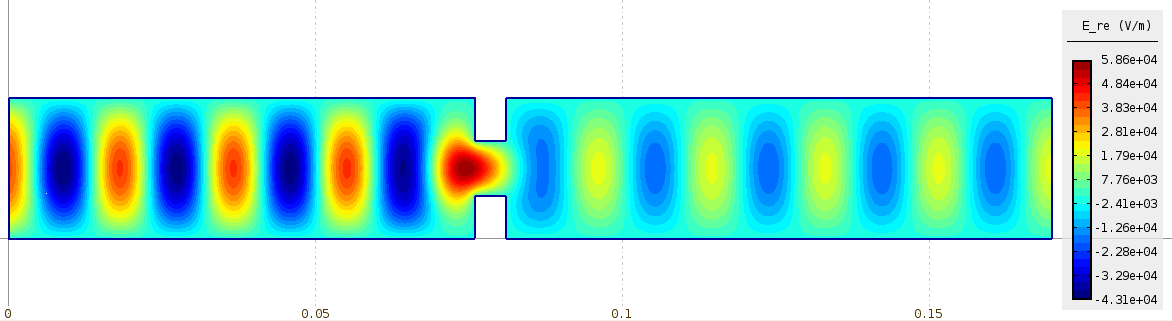
\includegraphics[width=15cm]{priklad_R100narrow_Ere_17Ghz.png}
	\caption{Rozložení $E_{z\Re}$ pro $f_3 = 17,5\unit{Ghz}$.}
	\label{obr:priklad_R100narrow_Ere_17Ghz}
\end{figure}

\newpage
\subsubsection*{3D zobrazení reálné složky intenzity elektrického pole.}
\begin{figure}[!h]
	\centering
	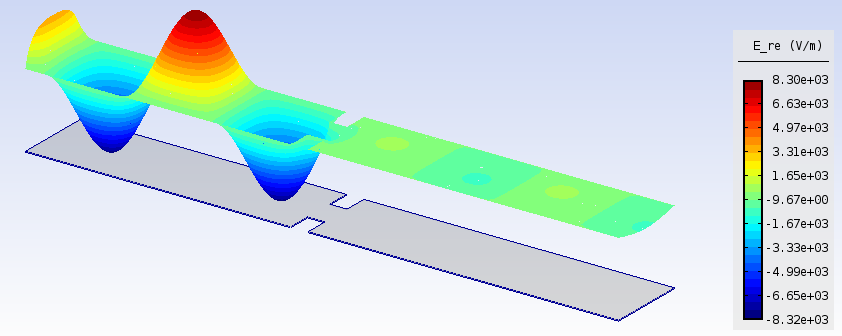
\includegraphics[width=14cm]{priklad_R100narrow_Ere_9Ghz_3D.png}
	\caption{Zobrazení $E_{z\Re}$ v prostoru pro $f_1 = 9\unit{Ghz}$.}
	\label{obr:priklad_R100narrow_Ere_9Ghz_3D}
\end{figure}
\begin{figure}[!h]
	\centering
	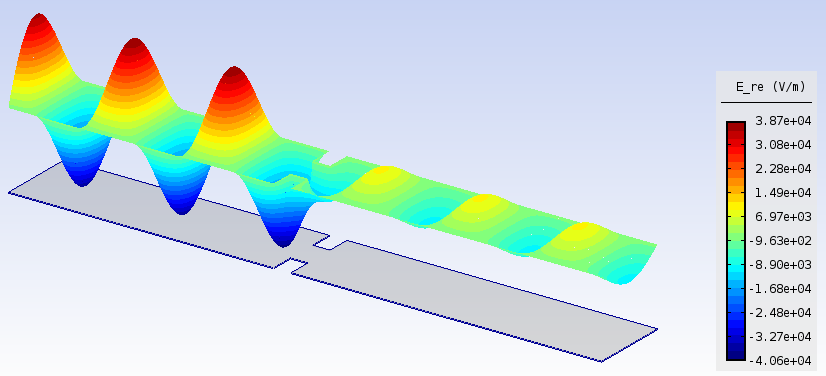
\includegraphics[width=14cm]{priklad_R100narrow_Ere_12Ghz_3D.png}
	\caption{Zobrazení $E_{z\Re}$ v prostoru pro $f_1 = 12,4\unit{Ghz}$.}
	\label{obr:priklad_R100narrow_Ere_12Ghz_3D}
\end{figure}
\begin{figure}[!h]
	\centering
	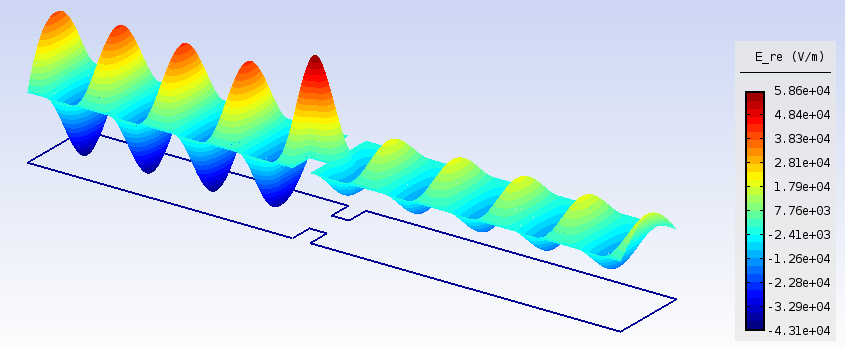
\includegraphics[width=14cm]{priklad_R100narrow_Ere_17Ghz_3D.png}
	\caption{Zobrazení $E_{z\Re}$ v prostoru pro $f_1 = 17,5\unit{Ghz}$.}
	\label{obr:priklad_R100narrow_Ere_17Ghz_3D}
\end{figure}